\chapter{Functions of Several variables}
\begin{thm}[23][Bananach's Fixed Point Theorem/Contraction Mapping Theorem]
	Let $(X,d)$ be a complete metric space. Suppose $\exists{c < 1} \text{ such that } $ the map $\phi:X\to X$ obeys $d(\phi(x),\phi(y))\le c d(x,y)$ for all $x,y \in X$ ($\phi$ is a \textit{ contraction }).
	Then $\exists{!} x \in X$ such that $\phi(x) = x$.
	\begin{proof}
		\begin{description}
			\item[Uniqueness:]
			      If $\phi(x)=x$ and $\phi(y)=y$, then $d(x,y)=d(\phi(x),\phi(y))\le c d(x,y)$, so $d(x,y)=0$ and $x=y$.
			\item[Existence:]
			      Given $x_{0} \in X$, let $x_{1}=\phi(x_{0}),x_{2}=\phi(x_{1})=(\phi \circ \phi)(x_{0})$, $x_{n+1}=\phi(x_n)=\underbrace{(\phi \circ \phi)}_{n+1}(x_{0})$.
			      Then $d(x_{n+1},x_n)=d(\phi(x_n), \phi(x_{n-1}))\le c d(x_n,x_{n-1})$, so by induction, $d(x_{n+1},x_n)\le c^{n}d(x_{1},x_{0})$ and hence for $n>m$,
			      \[
				      d(x_n,x_m)\le \sum_{i=m+1}^{n}{d(x_i,x_{i-1})}\le \sum_{i=m+1}^{n}{c^{i-1}d(x_{1},x_{0})} \le \sum_{i=m+1}^{\infty}{c^{i-1}d(x_{1},x_{0})}=\frac{c^{m}}{1-c} d(x_{1},x_{0}).\]
			      Hence, $\{x_n\}$ is a Cauchy sequence. As $X$ is assumed to be complete, $\exists x \in X$ such that $x_n \to x$. Since $\phi$ is continuous $\phi(x)=\lim_{n\to \infty}{\phi(x_n)}=\lim_{n\to \infty}{x_{n+1}}=x$.
		\end{description}

	\end{proof}
	\begin{remark}
		\begin{enumerate}
			\item $\phi$ is uniformly continuous ( take $\delta=\epsilon$ ).
			\item The proof gives an exponentially convergent algorithm to find the fixed point.
			\item Visualization of the algorithm used in the proof:\\
			      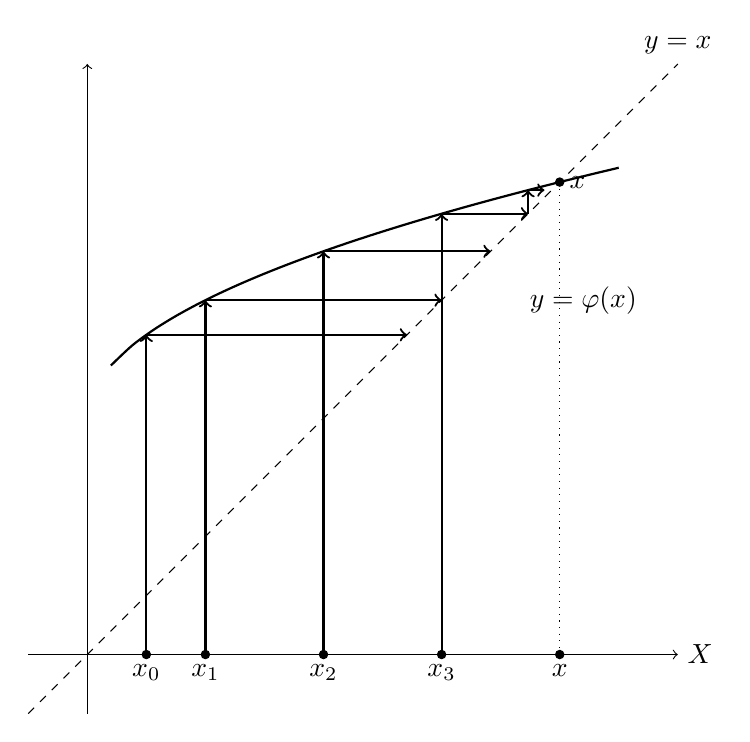
\begin{tikzpicture}[scale=1.5]
				      % Axes
				      \draw[->] (-0.5,0) -- (5,0) node[right] {$X$};
				      \draw[->] (0,-0.5) -- (0,5) node[above] {};

				      % y = x line
				      \draw[dashed] (-0.5,-0.5) -- (5,5) node[above] {$y = x$};

				      % Curve for y = \varphi(x)
				      \draw[thick, domain=0.2:4.5, smooth, variable=\x] plot ({\x},{sqrt(\x)+2});
				      \node at (4.2,3) {$y = \varphi(x)$};

				      % Points x0, x1, x2, x3, etc.
				      \foreach \x/\y/\name in {
				      0.5/{sqrt(0.5)+2}/x_0,
				      1/{sqrt(1)+2}/x_1,
				      2/{sqrt(2)+2}/x_2,
				      3/{sqrt(3)+2}/x_3
				      }{
				      \filldraw (\x,0) circle (1pt) node[below] {$\name$};
				      \draw[thick, ->] ({\x},0) -- ({\x},{\y});
				      \draw[thick, ->] ({\x},{\y}) -- ({\y},{\y});
				      }
				      % Converging to fixed point
				      \filldraw (4,{sqrt(4)+2}) circle (1pt);
				      \node[right] at (4,{sqrt(4)+2}) {$x$};

				      % Dotted line to x axis
				      \draw[thick, ->] ({sqrt(3)+2},{sqrt(3)+2}) -- ({sqrt(3)+2},{sqrt(sqrt(3)+2)+2});
				      \draw[thick, ->] ({sqrt(3)+2},{sqrt(sqrt(3)+2)+2}) -- ({sqrt(3.5)+2},{sqrt(sqrt(3)+2)+2});
				      % Labels
				      \node[below] at (4,0) {$x$};
				      \draw[dotted] (4,4) -- (4,0);
				      \filldraw (4,0) circle (1pt);

			      \end{tikzpicture}
		\end{enumerate}
		\item Reading assignment: Rudin's theorems 9.1-9.9.
	\end{remark}
\end{thm}

\section{Diffrentiation of functions of $f: \R^{n} \to \R^{m}$}

Recall for $n=m=1$,
\[
	f'(x)=\lim_{h\to \infty}{\frac{f(x+h)-f(x)}{h}}
	.\]

Equivalently, \[
	\lim_{h\to 0}{\left|\frac{f(x+h)-f(x)-f'(x)h}{h}\right|}=0
	.\]
This again is equivalent to
\[
	f(x+h)=f(x)+\underbrace{f'(x) h}_{\text{ best linear approximation to $f(x+h)-f(x)$ } }+\underbrace{r(h)}_{r(h)=o(h)}
	,\]
with $\lim_{h\to 0}{\frac{r(h)}{h}}=0$.


\begin{define}[11]
	Let $m,n \in \N$, $E \subset \R^{n}$ an open set, $f: E\to \R^{m}, x \in E$.
	Then $f$ is \textit{differentiable} at $x$ and $f'(x)=A$ if
	\[
		\lim_{h\to 0}{\frac{\|f(x+h)-f(x)-Ah\|}{\|h\|}}=0
		,\] where $A$ depends on $x$, $A \in L(\R^{n},\R^{m})$.
	Note $L(\R^{n},\R^{m})$ is the vector space of linear maps from $\R^{n}$ to $\R^{m}$.
	That is, if $f(x+h)=f(x)+Ah+r(h)$ with $\lim_{h\to 0}{\frac{\|r(h)\|}{\|h\|}}=0$.
\end{define}


\begin{thm}[12]
	$A$ in the definition of differentiability is unique if it exists.
	\begin{proof}
		Suppose
		\begin{flalign*}
			f(x+h) & =f(x)+A_{1}h + r_{1}(h) \\
			f(x+h) & =f(x)+A_{2}h + r_{2}(h) \\
			.\end{flalign*}
		with $r_{1}h=o(h), r_{2}h=o(h)$.
		Let $B=A_{1}-A_{2}$. Then $Bh=r_{2}(h)-r_{1}(h)$, so for a fixed $h\neq 0$ and $t>0$, \[
			\frac{\left|Bh\right|}{\left|h\right|}= \frac{\left|B(th)\right|}{\left|th\right|} \le \frac{\left|r_{2}(th)\right|}{th}+\frac{\left|r_{1}(th)\right|}{th}.\]
		$\frac{\left|Bh\right|}{\left|h\right|}$ is independent of $t$. Hence, $\frac{\left|Bh\right|}{\left|h\right|}\to 0$ as $h\to 0$ (think of $th=h'\to 0$).
		$Bh=0$ for all $h \in \R^{n}$; i.e., $B=0$; i.e., $A_{1}=A_{2}$.
	\end{proof}
	\begin{note}
		\begin{enumerate}
			\item If $f'(x)$ exists for all $x \in E$ then we can regard $f'$ as a function $f':E\to L(\R^{n},\R^{m})$.
			\item Suppose $f: \R^{n}\to \R^{m}$ is linear. Then $f(x+h)=f(x)+\underbrace{f(h)}_{=Ah \text{ with } A=f}+0$ for all $x,h \in \R^{n}$.
			      Hence, $f'(x)=f(x)$ for all $x \in \R^{n}$.\\
			      For $n=m=1$, we can identify a linear map $f: \R\to \R, f(x)=ax$ with $a \in \R$. Then $f'(x)=a$ is consistent with the above.
		\end{enumerate}
	\end{note}

\end{thm}


